\documentclass[11pt,a4paper]{article}
\usepackage[margin=0.8in]{geometry}
\usepackage{tikz}
\usepackage{pgf-umlcd}
\usepackage{fontspec}
\usepackage{xcolor}
\usepackage{amsfonts}
\usepackage{amsmath}
\usepackage{listings}

% Configure emoji font for XeLaTeX (vector-based for better compatibility)
\newfontfamily\emojifont{Segoe UI Emoji}[
    Scale=1.0
]

% Fallback emoji font if Segoe UI Emoji is not available
% \newfontfamily\emojifont{TwemojiMozilla.ttf}[Scale=1.0]

% Create convenient emoji command
\newcommand{\emoji}[1]{{\emojifont #1}}

\usetikzlibrary{shapes,arrows,positioning,fit,backgrounds,decorations.pathmorphing,calc,shadows,matrix,chains}

\title{PeiDocker Terminal GUI - Simple Mode Wizard Design}
\author{Claude Code}
\date{\today}

\definecolor{primaryblue}{RGB}{51,122,183}
\definecolor{successgreen}{RGB}{92,184,92}
\definecolor{warningorange}{RGB}{240,173,78}
\definecolor{dangered}{RGB}{217,83,79}
\definecolor{lightgray}{RGB}{248,248,248}
\definecolor{darkgray}{RGB}{85,85,85}
\definecolor{infoblue}{RGB}{91,192,222}

\tikzset{
    % Screen frame style
    screen/.style={
        rectangle, draw=primaryblue, thick, fill=lightgray!30,
        minimum width=14cm, minimum height=10cm,
        rounded corners=5pt
    },
    % Input field style
    inputfield/.style={
        rectangle, draw=darkgray, fill=white,
        minimum width=6cm, minimum height=0.8cm,
        rounded corners=2pt
    },
    % Button styles
    primarybtn/.style={
        rectangle, draw=primaryblue, thick, fill=primaryblue!30,
        minimum width=2cm, minimum height=0.8cm,
        rounded corners=3pt, font=\bfseries
    },
    secondarybtn/.style={
        rectangle, draw=darkgray, fill=lightgray,
        minimum width=2cm, minimum height=0.8cm,
        rounded corners=3pt
    },
    % Label style
    label/.style={
        rectangle, draw=none, fill=none,
        font=\bfseries, anchor=west
    },
    % Help text style
    helptext/.style={
        rectangle, draw=infoblue, fill=infoblue!10,
        text width=12cm, rounded corners=3pt,
        font=\footnotesize
    },
    % Warning style
    warning/.style={
        rectangle, draw=warningorange, fill=warningorange!20,
        text width=12cm, rounded corners=3pt,
        font=\footnotesize
    },
    % Navigation arrows
    navarrow/.style={
        ->, >=stealth, thick, color=primaryblue
    }
}

\begin{document}

\maketitle

\section{Simple Mode Wizard Flow Overview}

The Simple Mode provides a step-by-step wizard interface that guides users through creating a basic PeiDocker configuration. The wizard consists of 15 main steps, each focusing on a specific aspect of the container configuration.

\subsection{Wizard Flow Diagram}

\begin{figure}[htbp]
\centering
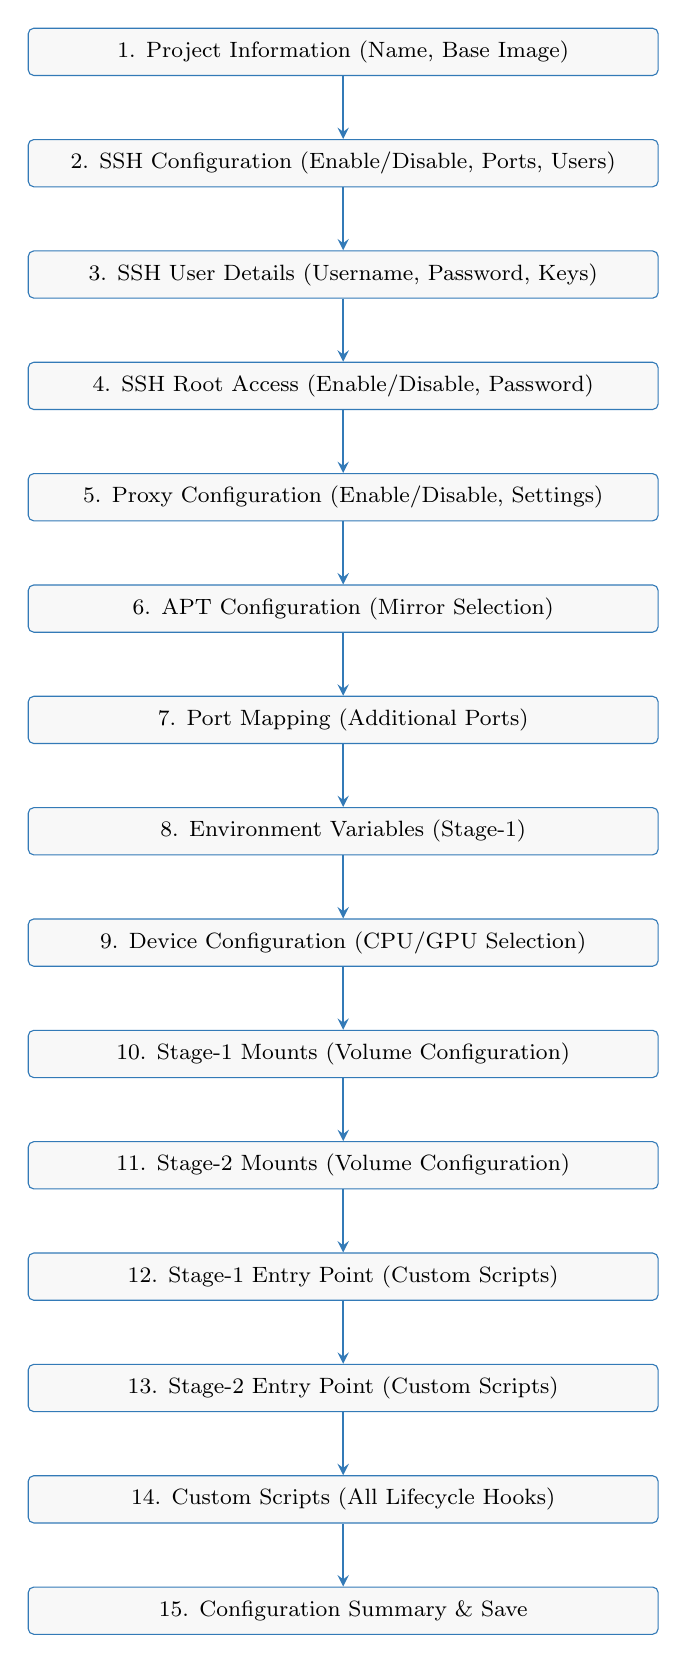
\begin{tikzpicture}[
    start chain=going below,
    node distance=0.8cm,
    every node/.style={on chain},
    wizardstep/.style={
        rectangle, draw=primaryblue, fill=lightgray,
        minimum width=8cm, minimum height=0.6cm,
        rounded corners=2pt, font=\footnotesize
    }
]

\node[wizardstep] {1. Project Information (Name, Base Image)};
\node[wizardstep] {2. SSH Configuration (Enable/Disable, Ports, Users)};
\node[wizardstep] {3. SSH User Details (Username, Password, Keys)};
\node[wizardstep] {4. SSH Root Access (Enable/Disable, Password)};
\node[wizardstep] {5. Proxy Configuration (Enable/Disable, Settings)};
\node[wizardstep] {6. APT Configuration (Mirror Selection)};
\node[wizardstep] {7. Port Mapping (Additional Ports)};
\node[wizardstep] {8. Environment Variables (Stage-1)};
\node[wizardstep] {9. Device Configuration (CPU/GPU Selection)};
\node[wizardstep] {10. Stage-1 Mounts (Volume Configuration)};
\node[wizardstep] {11. Stage-2 Mounts (Volume Configuration)};
\node[wizardstep] {12. Stage-1 Entry Point (Custom Scripts)};
\node[wizardstep] {13. Stage-2 Entry Point (Custom Scripts)};
\node[wizardstep] {14. Custom Scripts (All Lifecycle Hooks)};
\node[wizardstep] {15. Configuration Summary \& Save};

% Add navigation arrows
\foreach \i in {1,...,14} {
    \draw[navarrow] (chain-\i) -- (chain-\the\numexpr\i+1\relax);
}

\end{tikzpicture}
\caption{Complete Simple Mode Wizard Flow}
\end{figure}

\section{Individual Screen Designs}

\subsection{Step 1: Project Information}

\begin{figure}[htbp]
\centering
\begin{tikzpicture}

% Main screen frame
\node[screen] (frame) at (0,0) {};
\node[anchor=north] at (0,4.7) {\Large\textbf{PeiDocker Simple Wizard - Step 1/15}};

% Progress bar
\draw[fill=primaryblue!30] (-6.5,4) rectangle (6.5,4.3);
\draw[fill=primaryblue] (-6.5,4) rectangle (-5.6,4.3);
\node[font=\footnotesize] at (0,4.15) {Project Information - 1 of 15 steps};

% Project name input
\node[label] at (-6,2.5) {Project Name:};
\node[inputfield] (projname) at (-2,2.5) {};
\node[anchor=west, font=\ttfamily] at (-5,2.5) {my\_awesome\_project};

\node[helptext] at (0,1.5) {
    Enter a name for your project. This will be used as the Docker image name\\
    (e.g., my\_awesome\_project:stage-1, my\_awesome\_project:stage-2)\\
    \textbf{Note:} If Docker is available, we'll check for existing images with this name.
};

% Base image input
\node[label] at (-6,0.5) {Base Image:};
\node[inputfield] (baseimage) at (-2,0.5) {};
\node[anchor=west, font=\ttfamily] at (-5,0.5) {ubuntu:24.04};

\node[helptext] at (0,-0.5) {
    Enter the Docker base image tag from Docker Hub\\
    \textbf{Default:} ubuntu:24.04 (recommended for most users)
};

% Warning area (conditional)
\node[warning] at (0,-2) {
    \textbf{\emoji{\emoji{⚠}} Warning:} Docker image "my\_awesome\_project:stage-1" already exists.\\
    Continuing will overwrite the existing image.
};

% Navigation buttons
\node[secondarybtn] at (-3,-4) {Back};
\node[primarybtn] at (0,-4) {Next};
\node[secondarybtn] at (3,-4) {Cancel};

% Navigation help
\node[font=\footnotesize, color=darkgray] at (0,-4.7) {TAB: Navigate fields | ENTER: Next | ESC: Cancel};

\end{tikzpicture}
\caption{Step 1: Project Information Screen}
\end{figure}

\subsection{Step 2: SSH Configuration}

\begin{figure}[htbp]
\centering
\begin{tikzpicture}

\node[screen] (frame) at (0,0) {};
\node[anchor=north] at (0,4.7) {\Large\textbf{PeiDocker Simple Wizard - Step 2/15}};

% Progress bar
\draw[fill=primaryblue!30] (-6.5,4) rectangle (6.5,4.3);
\draw[fill=primaryblue] (-6.5,4) rectangle (-5.2,4.3);
\node[font=\footnotesize] at (0,4.15) {SSH Configuration - 2 of 15 steps};

% SSH Enable/Disable
\node[label] at (-6,3) {Enable SSH Access:};
\draw[fill=successgreen] (-4.5,2.8) rectangle (-4.2,3.2);
\node[font=\footnotesize] at (-3.5,3) {\emoji{✓} Yes (Recommended)};
\draw (-2.5,2.8) rectangle (-2.2,3.2);
\node[font=\footnotesize] at (-1.5,3) {No};

% Container port
\node[label] at (-6,2) {SSH Container Port:};
\node[inputfield] (sshport) at (-2,2) {};
\node[anchor=west, font=\ttfamily] at (-5,2) {22};

% Host port
\node[label] at (-6,1) {SSH Host Port:};
\node[inputfield] (hostport) at (-2,1) {};
\node[anchor=west, font=\ttfamily] at (-5,1) {2222};

\node[helptext] at (0,0) {
    \textbf{SSH Container Port:} Port inside the container (default: 22)\\
    \textbf{SSH Host Port:} Port on your machine to access the container (default: 2222)\\
    \textbf{Example:} ssh -p 2222 username@localhost
};

% Warning for no SSH
\node[warning] at (0,-1.5) {
    \textbf{\emoji{⚠} Warning:} If you disable SSH, you'll need to use native Docker commands\\
    like "docker exec -it container\_name bash" to access the container.
};

% Navigation buttons
\node[secondarybtn] at (-3,-4) {Back};
\node[primarybtn] at (0,-4) {Next};
\node[secondarybtn] at (3,-4) {Cancel};

\end{tikzpicture}
\caption{Step 2: SSH Configuration Screen}
\end{figure}

\subsection{Step 3: SSH User Configuration}

\begin{figure}[htbp]
\centering
\begin{tikzpicture}

\node[screen] (frame) at (0,0) {};
\node[anchor=north] at (0,4.7) {\Large\textbf{PeiDocker Simple Wizard - Step 3/15}};

% Progress bar
\draw[fill=primaryblue!30] (-6.5,4) rectangle (6.5,4.3);
\draw[fill=primaryblue] (-6.5,4) rectangle (-4.8,4.3);

% Username
\node[label] at (-6,3) {SSH Username:};
\node[inputfield] at (-2,3) {};
\node[anchor=west, font=\ttfamily] at (-5,3) {me};

% Password
\node[label] at (-6,2.2) {SSH Password:};
\node[inputfield] at (-2,2.2) {};
\node[anchor=west, font=\ttfamily] at (-5,2.2) {123456};

\node[warning] at (0,1.4) {
    \textbf{\emoji{⚠} Important:} Do not use commas (,) or spaces in passwords\\
    due to implementation limitations.
};

% Public key option
\node[label] at (-6,0.5) {Specify Public Key:};
\draw (-4.5,0.3) rectangle (-4.2,0.7);
\node[font=\footnotesize] at (-3.5,0.5) {No};
\draw[fill=successgreen] (-2.5,0.3) rectangle (-2.2,0.7);
\node[font=\footnotesize] at (-1.5,0.5) {\emoji{✓} Yes};

% Key input (shown when Yes selected)
\node[inputfield] at (2,-0.2) {};
\node[anchor=west, font=\ttfamily, color=darkgray] at (-1,-0.2) {Enter public key or "~" for auto-discovery};

% Private key option
\node[label] at (-6,-1) {Specify Private Key:};
\draw[fill=successgreen] (-4.5,-1.2) rectangle (-4.2,-0.8);
\node[font=\footnotesize] at (-3.5,-1) {\emoji{✓} No};
\draw (-2.5,-1.2) rectangle (-2.2,-0.8);
\node[font=\footnotesize] at (-1.5,-1) {Yes};

\node[helptext] at (0,-2.2) {
    \textbf{Public Key:} Enter key content or "~" for system key discovery\\
    \textbf{Private Key:} Enter file path or "~" for system key discovery\\
    \textbf{Note:} Keys are optional if password authentication is enabled
};

% Navigation buttons
\node[secondarybtn] at (-3,-4) {Back};
\node[primarybtn] at (0,-4) {Next};
\node[secondarybtn] at (3,-4) {Cancel};

\end{tikzpicture}
\caption{Step 3: SSH User Configuration Screen}
\end{figure}

\subsection{Step 4: SSH Root Access}

\begin{figure}[htbp]
\centering
\begin{tikzpicture}

\node[screen] (frame) at (0,0) {};
\node[anchor=north] at (0,4.7) {\Large\textbf{PeiDocker Simple Wizard - Step 4/15}};

% Progress bar
\draw[fill=primaryblue!30] (-6.5,4) rectangle (6.5,4.3);
\draw[fill=primaryblue] (-6.5,4) rectangle (-4.4,4.3);

% Root SSH access
\node[label] at (-6,2.5) {Allow Root SSH Access:};
\draw[fill=successgreen] (-4.5,2.3) rectangle (-4.2,2.7);
\node[font=\footnotesize] at (-3.5,2.5) {\emoji{✓} No (Recommended)};
\draw (-2.5,2.3) rectangle (-2.2,2.7);
\node[font=\footnotesize] at (-1.5,2.5) {Yes};

% Root password (shown when Yes selected)
\node[label] at (-6,1.5) {Root Password:};
\node[inputfield] at (-2,1.5) {};
\node[anchor=west, font=\ttfamily] at (-5,1.5) {root};

\node[helptext] at (0,0.7) {
    \textbf{Security Note:} Root SSH access is generally not recommended.\\
    Use your regular user account and sudo for administrative tasks.
};

\node[warning] at (0,-0.5) {
    \textbf{\emoji{⚠} Security Warning:} Enabling root SSH access reduces security.\\
    Only enable if absolutely necessary for your use case.\\
    \textbf{Note:} SSH keys cannot be configured for root in Simple Mode.
};

% Navigation buttons
\node[secondarybtn] at (-3,-4) {Back};
\node[primarybtn] at (0,-4) {Next};
\node[secondarybtn] at (3,-4) {Cancel};

\end{tikzpicture}
\caption{Step 4: SSH Root Access Screen}
\end{figure}

\subsection{Step 5: Proxy Configuration}

\begin{figure}[htbp]
\centering
\begin{tikzpicture}

\node[screen] (frame) at (0,0) {};
\node[anchor=north] at (0,4.7) {\Large\textbf{PeiDocker Simple Wizard - Step 5/15}};

% Progress bar
\draw[fill=primaryblue!30] (-6.5,4) rectangle (6.5,4.3);
\draw[fill=primaryblue] (-6.5,4) rectangle (-4,4.3);

% Proxy enable
\node[label] at (-6,3) {Use Host Proxy:};
\draw[fill=successgreen] (-4.5,2.8) rectangle (-4.2,3.2);
\node[font=\footnotesize] at (-3.5,3) {\emoji{✓} No};
\draw (-2.5,2.8) rectangle (-2.2,3.2);
\node[font=\footnotesize] at (-1.5,3) {Yes};

% Proxy port (shown when Yes selected)
\node[label] at (-6,2) {Proxy Port:};
\node[inputfield] at (-2,2) {};
\node[anchor=west, font=\ttfamily] at (-5,2) {7890};

% Build-only option
\node[label] at (-6,1) {Use Only During Build:};
\draw[fill=successgreen] (-4.5,0.8) rectangle (-4.2,1.2);
\node[font=\footnotesize] at (-3.5,1) {\emoji{✓} Yes (Recommended)};
\draw (-2.5,0.8) rectangle (-2.2,1.2);
\node[font=\footnotesize] at (-1.5,1) {No};

\node[helptext] at (0,0) {
    \textbf{Proxy Configuration:} This will set http\_proxy and https\_proxy environment variables\\
    \textbf{Build Only:} Proxy removed after build (recommended for production)\\
    \textbf{Runtime:} Proxy available during container runtime (affects running applications)
};

\node[helptext] at (0,-1.5) {
    \textbf{Note:} The proxy address will be automatically set to host.docker.internal\\
    to allow the container to access your host machine's proxy service.
};

% Navigation buttons
\node[secondarybtn] at (-3,-4) {Back};
\node[primarybtn] at (0,-4) {Next};
\node[secondarybtn] at (3,-4) {Cancel};

\end{tikzpicture}
\caption{Step 5: Proxy Configuration Screen}
\end{figure}

\subsection{Step 6: APT Configuration}

\begin{figure}[htbp]
\centering
\begin{tikzpicture}

\node[screen] (frame) at (0,0) {};
\node[anchor=north] at (0,4.7) {\Large\textbf{PeiDocker Simple Wizard - Step 6/15}};

% Progress bar
\draw[fill=primaryblue!30] (-6.5,4) rectangle (6.5,4.3);
\draw[fill=primaryblue] (-6.5,4) rectangle (-3.6,4.3);

% APT mirror selection
\node[label] at (-6,3.5) {Use Different APT Mirror:};
\draw[fill=successgreen] (-4.5,3.3) rectangle (-4.2,3.7);
\node[font=\footnotesize] at (-3.5,3.5) {\emoji{✓} No (Use Default)};
\draw (-2.5,3.3) rectangle (-2.2,3.7);
\node[font=\footnotesize] at (-1.5,3.5) {Yes};

% Mirror selection dropdown (shown when Yes selected)
\node[label] at (-6,2.5) {Select Mirror:};
\draw[draw=darkgray, fill=white] (-4,2.3) rectangle (1,2.7);
\node[anchor=west, font=\ttfamily] at (-3.8,2.5) {tuna (Tsinghua University) \emoji{▼}};

% Mirror options list
\draw[draw=darkgray, fill=white] (-4,0.5) rectangle (1,2.2);
\node[anchor=west, font=\footnotesize] at (-3.8,2) {\emoji{✓} tuna - Tsinghua University mirror};
\node[anchor=west, font=\footnotesize] at (-3.8,1.7) {aliyun - Aliyun mirror};
\node[anchor=west, font=\footnotesize] at (-3.8,1.4) {163 - 163 mirror};
\node[anchor=west, font=\footnotesize] at (-3.8,1.1) {ustc - USTC mirror};
\node[anchor=west, font=\footnotesize] at (-3.8,0.8) {cn - Ubuntu official China mirror};
\node[anchor=west, font=\footnotesize] at (-3.8,0.5) {default - Standard Ubuntu mirror};

\node[helptext] at (0,-0.8) {
    \textbf{APT Mirrors:} Alternative package sources for faster downloads\\
    \textbf{Recommended for Chinese users:} tuna, aliyun, or ustc mirrors\\
    \textbf{Default:} Standard Ubuntu repositories (works worldwide)
};

% Navigation buttons
\node[secondarybtn] at (-3,-4) {Back};
\node[primarybtn] at (0,-4) {Next};
\node[secondarybtn] at (3,-4) {Cancel};

\end{tikzpicture}
\caption{Step 6: APT Configuration Screen}
\end{figure}

\subsection{Step 7-8: Port Mapping \& Environment Variables}

\begin{figure}[htbp]
\centering
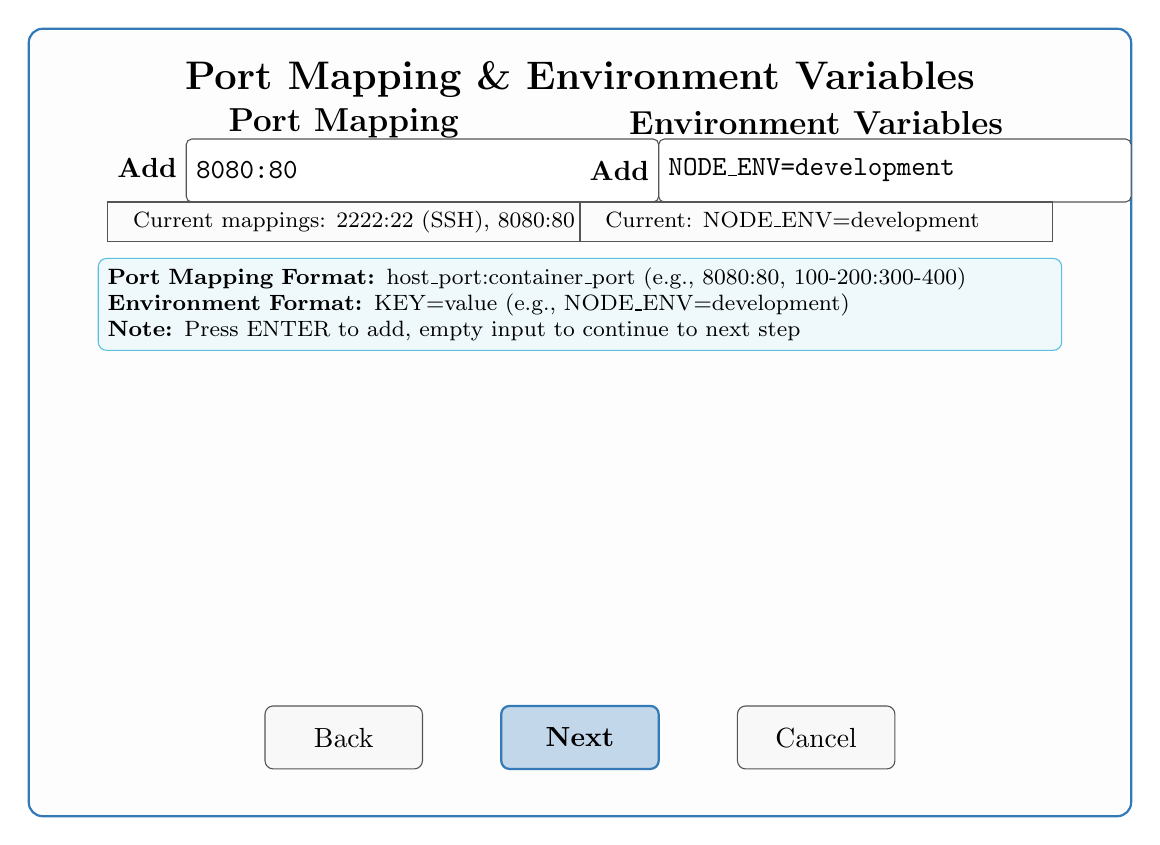
\begin{tikzpicture}

\node[screen] (frame) at (0,0) {};
\node[anchor=north] at (0,4.7) {\Large\textbf{Port Mapping \& Environment Variables}};

% Port mapping section
\node[font=\large\bfseries] at (-3,3.8) {Port Mapping};
\node[label] at (-6,3.2) {Add Port Mapping:};
\node[inputfield] at (-2,3.2) {};
\node[anchor=west, font=\ttfamily] at (-5,3.2) {8080:80};

% Current mappings list
\draw[draw=darkgray, fill=lightgray!50] (-6,2.3) rectangle (0,2.8);
\node[anchor=west, font=\footnotesize] at (-5.8,2.55) {Current mappings: 2222:22 (SSH), 8080:80};

% Environment variables section
\node[font=\large\bfseries] at (3,3.8) {Environment Variables};
\node[label] at (0,3.2) {Add Variable:};
\node[inputfield] at (4,3.2) {};
\node[anchor=west, font=\ttfamily] at (1,3.2) {NODE\_ENV=development};

% Current variables list
\draw[draw=darkgray, fill=lightgray!50] (0,2.3) rectangle (6,2.8);
\node[anchor=west, font=\footnotesize] at (0.2,2.55) {Current: NODE\_ENV=development};

\node[helptext] at (0,1.5) {
    \textbf{Port Mapping Format:} host\_port:container\_port (e.g., 8080:80, 100-200:300-400)\\
    \textbf{Environment Format:} KEY=value (e.g., NODE\_ENV=development)\\
    \textbf{Note:} Press ENTER to add, empty input to continue to next step
};

% Navigation buttons
\node[secondarybtn] at (-3,-4) {Back};
\node[primarybtn] at (0,-4) {Next};
\node[secondarybtn] at (3,-4) {Cancel};

\end{tikzpicture}
\caption{Step 7-8: Port Mapping \& Environment Variables}
\end{figure}

\subsection{Step 9: Device Configuration}

\begin{figure}[htbp]
\centering
\begin{tikzpicture}

\node[screen] (frame) at (0,0) {};
\node[anchor=north] at (0,4.7) {\Large\textbf{PeiDocker Simple Wizard - Step 9/15}};

% Progress bar
\draw[fill=primaryblue!30] (-6.5,4) rectangle (6.5,4.3);
\draw[fill=primaryblue] (-6.5,4) rectangle (-2.8,4.3);

% GPU selection
\node[label] at (-6,2.5) {Use GPU Acceleration:};
\draw[fill=successgreen] (-4.5,2.3) rectangle (-4.2,2.7);
\node[font=\footnotesize] at (-3.5,2.5) {\emoji{✓} No (CPU Only)};
\draw (-2.5,2.3) rectangle (-2.2,2.7);
\node[font=\footnotesize] at (-1.5,2.5) {Yes (GPU)};

\node[helptext] at (0,1.5) {
    \textbf{CPU Mode:} Standard processing using CPU resources\\
    \textbf{GPU Mode:} Enables NVIDIA GPU support for CUDA workloads\\
    \textbf{Note:} GPU mode requires NVIDIA Docker runtime and compatible hardware
};

\node[warning] at (0,0.3) {
    \textbf{\emoji{⚠} Important:} We do not automatically detect GPU availability.\\
    Only select GPU mode if you have NVIDIA GPUs and Docker GPU support installed.\\
    Incorrect selection may cause container startup failures.
};

\node[helptext] at (0,-1) {
    \textbf{Prerequisites for GPU mode:}\\
    • NVIDIA GPU with recent drivers\\
    • nvidia-container-toolkit installed\\
    • Docker configured for GPU support
};

% Navigation buttons
\node[secondarybtn] at (-3,-4) {Back};
\node[primarybtn] at (0,-4) {Next};
\node[secondarybtn] at (3,-4) {Cancel};

\end{tikzpicture}
\caption{Step 9: Device Configuration Screen}
\end{figure}

\subsection{Steps 10-11: Mount Configuration}

\begin{figure}[htbp]
\centering
\begin{tikzpicture}

\node[screen] (frame) at (0,0) {};
\node[anchor=north] at (0,4.7) {\Large\textbf{Additional Mounts Configuration}};

% Stage selection
\node[font=\large\bfseries] at (0,3.8) {Stage-1 Mounts Configuration};

% Add mount question
\node[label] at (-6,3) {Add Additional Mounts:};
\draw[fill=successgreen] (-4.5,2.8) rectangle (-4.2,3.2);
\node[font=\footnotesize] at (-3.5,3) {\emoji{✓} No};
\draw (-2.5,2.8) rectangle (-2.2,3.2);
\node[font=\footnotesize] at (-1.5,3) {Yes};

% Mount type selection (shown when Yes)
\node[label] at (-6,2) {Mount Type:};
\draw[draw=darkgray, fill=white] (-4,1.8) rectangle (1,2.2);
\node[anchor=west, font=\ttfamily] at (-3.8,2) {Automatic Docker Volume \emoji{▼}};

% Mount type options
\draw[draw=darkgray, fill=white] (-4,0.5) rectangle (2,1.7);
\node[anchor=west, font=\footnotesize] at (-3.8,1.5) {\emoji{✓} Automatic Docker Volume};
\node[anchor=west, font=\footnotesize] at (-3.8,1.2) {Manual Docker Volume};
\node[anchor=west, font=\footnotesize] at (-3.8,0.9) {Host Directory};
\node[anchor=west, font=\footnotesize] at (-3.8,0.6) {Done (finish mounting)};

% Mount details (conditional)
\node[label] at (3,2) {Destination Path:};
\node[inputfield] at (5.5,2) {};
\node[anchor=west, font=\ttfamily] at (3.2,2) {/data};

\node[label] at (3,1.5) {Volume Name:};
\node[inputfield] at (5.5,1.5) {};
\node[anchor=west, font=\ttfamily] at (3.2,1.5) {myproject\_data};

\node[helptext] at (0,-0.5) {
    \textbf{Automatic Volume:} Docker manages the volume automatically\\
    \textbf{Manual Volume:} You specify the volume name\\
    \textbf{Host Directory:} Mount a directory from your host machine\\
    \textbf{Note:} Stage-2 mounts will completely override Stage-1 mounts
};

% Navigation buttons
\node[secondarybtn] at (-3,-4) {Back};
\node[primarybtn] at (0,-4) {Next};
\node[secondarybtn] at (3,-4) {Cancel};

\end{tikzpicture}
\caption{Steps 10-11: Mount Configuration Screen}
\end{figure}

\subsection{Steps 12-13: Entry Point Configuration}

\begin{figure}[htbp]
\centering
\begin{tikzpicture}

\node[screen] (frame) at (0,0) {};
\node[anchor=north] at (0,4.7) {\Large\textbf{Custom Entry Point Configuration}};

% Stage selection
\node[font=\large\bfseries] at (0,3.8) {Stage-1 Entry Point Configuration};

% Entry point question
\node[label] at (-6,3) {Set Custom Entry Point:};
\draw[fill=successgreen] (-4.5,2.8) rectangle (-4.2,3.2);
\node[font=\footnotesize] at (-3.5,3) {\emoji{✓} No (Use Default Shell)};
\draw (-2.5,2.8) rectangle (-2.2,3.2);
\node[font=\footnotesize] at (-1.5,3) {Yes (Custom Script)};

% Script path input (shown when Yes)
\node[label] at (-6,2) {Entry Point Script:};
\node[inputfield] at (-1.5,2) {};
\node[anchor=west, font=\ttfamily] at (-5.8,2) {/path/to/startup.sh};

\node[helptext] at (0,1) {
    \textbf{Entry Point Script:} Custom script to run when container starts\\
    \textbf{Format:} Path to .sh script file (relative to project directory)\\
    \textbf{Default Behavior:} Interactive shell startup if no custom entry point
};

\node[warning] at (0,0) {
    \textbf{\emoji{⚠} Important:} Stage-2 entry point will completely override Stage-1 entry point.\\
    The script file will be copied to the project directory if it exists.
};

\node[helptext] at (0,-1.2) {
    \textbf{Example Entry Points:}\\
    • stage-1/custom/my-startup.sh\\
    • scripts/init-environment.sh\\
    • Leave empty for default interactive shell
};

% Navigation buttons
\node[secondarybtn] at (-3,-4) {Back};
\node[primarybtn] at (0,-4) {Next};
\node[secondarybtn] at (3,-4) {Cancel};

\end{tikzpicture}
\caption{Steps 12-13: Entry Point Configuration Screen}
\end{figure}

\subsection{Step 14: Custom Scripts Configuration}

\begin{figure}[htbp]
\centering
\begin{tikzpicture}

\node[screen] (frame) at (0,0) {};
\node[anchor=north] at (0,4.7) {\Large\textbf{Custom Scripts Configuration}};

% Stage and script type
\node[font=\large\bfseries] at (0,3.8) {Stage-1: on\_build Scripts};

% Add scripts question
\node[label] at (-6,3.2) {Add Custom Scripts:};
\draw (-4.5,3) rectangle (-4.2,3.4);
\node[font=\footnotesize] at (-3.5,3.2) {No};
\draw[fill=successgreen] (-2.5,3) rectangle (-2.2,3.4);
\node[font=\footnotesize] at (-1.5,3.2) {\emoji{✓} Yes};

% Script description
\node[helptext] at (0,2.4) {
    \textbf{on\_build scripts:} Execute during Docker image build process\\
    These scripts can install packages, configure system settings, etc.
};

% Script input
\node[label] at (-6,1.5) {Script Path:};
\node[inputfield] at (-1.5,1.5) {};
\node[anchor=west, font=\ttfamily] at (-5.8,1.5) {stage-1/custom/install-tools.sh --verbose};

% Current scripts list
\node[label] at (-6,0.8) {Added Scripts:};
\draw[draw=darkgray, fill=lightgray!50] (-6,0.2) rectangle (6,0.7);
\node[anchor=west, font=\footnotesize] at (-5.8,0.45) {1. stage-1/custom/install-tools.sh --verbose};

% Script type navigation
\draw (-6,-0.5) rectangle (-3,-0.1);
\node[font=\footnotesize] at (-4.5,-0.3) {on\_build};
\draw (-2.5,-0.5) rectangle (0.5,-0.1);
\node[font=\footnotesize] at (-1,-0.3) {on\_first\_run};
\draw (1,-0.5) rectangle (4,-0.1);
\node[font=\footnotesize] at (2.5,-0.3) {on\_every\_run};
\draw (4.5,-0.5) rectangle (6.5,-0.1);
\node[font=\footnotesize] at (5.5,-0.3) {on\_user\_login};

\node[helptext] at (0,-1.5) {
    \textbf{Script Types:}\\
    \textbf{on\_build:} Run during image build • \textbf{on\_first\_run:} Run on first container start\\
    \textbf{on\_every\_run:} Run on every start • \textbf{on\_user\_login:} Run when user logs in via SSH\\
    \textbf{Format:} script\_path --arg1 value1 --arg2 "value with spaces"
};

% Navigation buttons
\node[secondarybtn] at (-3,-4) {Back};
\node[primarybtn] at (0,-4) {Next};
\node[secondarybtn] at (3,-4) {Cancel};

\end{tikzpicture}
\caption{Step 14: Custom Scripts Configuration Screen}
\end{figure}

\subsection{Step 15: Configuration Summary}

\begin{figure}[htbp]
\centering
\begin{tikzpicture}

\node[screen] (frame) at (0,0) {};
\node[anchor=north] at (0,4.7) {\Large\textbf{Configuration Summary \& Save}};

% Progress bar - complete
\draw[fill=primaryblue] (-6.5,4) rectangle (6.5,4.3);
\node[font=\footnotesize, color=white] at (0,4.15) {Configuration Complete - 15 of 15 steps};

% Summary sections
\node[font=\bfseries] at (-5,3.5) {Project Configuration Summary:};

% Left column
\draw[draw=darkgray, fill=lightgray!30] (-6.5,1.5) rectangle (-0.5,3.3);
\node[anchor=north west, font=\footnotesize, text width=5.5cm, align=left] at (-6.3,3.2) {
    \textbf{Project:} my\_awesome\_project\\
    \textbf{Base Image:} ubuntu:24.04\\
    \textbf{SSH:} Enabled (user: me, port: 2222)\\
    \textbf{Proxy:} Disabled\\
    \textbf{APT Mirror:} tuna (Tsinghua)\\
    \textbf{Ports:} 2222:22, 8080:80\\
    \textbf{Environment:} NODE\_ENV=development
};

% Right column
\draw[draw=darkgray, fill=lightgray!30] (0.5,1.5) rectangle (6.5,3.3);
\node[anchor=north west, font=\footnotesize, text width=5.5cm, align=left] at (0.7,3.2) {
    \textbf{Device:} CPU Only\\
    \textbf{Stage-1 Mounts:} /data (auto-volume)\\
    \textbf{Stage-2 Mounts:} None\\
    \textbf{Entry Points:} Default shell\\
    \textbf{Custom Scripts:} 2 on\_build scripts\\
    \textbf{Estimated Build Time:} 5-10 minutes
};

% Save options
\node[font=\bfseries] at (0,1) {Save Configuration:};
\draw[fill=successgreen] (-2,0.5) rectangle (-1.7,0.9);
\node[font=\footnotesize] at (-1,0.7) {\emoji{✓} Save and return to main menu};
\draw (0,0.5) rectangle (0.3,0.9);
\node[font=\footnotesize] at (1.2,0.7) {Save and start build process};
\draw (3,0.5) rectangle (3.3,0.9);
\node[font=\footnotesize] at (4.2,0.7) {Discard and return to main menu};

\node[helptext] at (0,-0.5) {
    \textbf{Next Steps After Saving:}\\
    1. Run: cd /path/to/my\_project \quad 2. Run: pei-docker-cli configure\\
    3. Run: docker compose build stage-1 \quad 4. Run: docker compose build stage-2\\
    5. Run: docker compose up stage-2 \quad 6. Connect: ssh -p 2222 me@localhost
};

% Navigation buttons
\node[secondarybtn] at (-3,-4) {Back};
\node[primarybtn] at (0,-4) {Save \& Exit};
\node[secondarybtn] at (3,-4) {Cancel};

\end{tikzpicture}
\caption{Step 15: Configuration Summary \& Save Screen}
\end{figure}

\section{Navigation and Interaction Patterns}

\subsection{Common UI Elements}

\begin{itemize}
    \item \textbf{Progress Bar}: Shows current step and overall progress
    \item \textbf{Navigation Buttons}: Back, Next/Save, Cancel consistently placed
    \item \textbf{Keyboard Shortcuts}: TAB (navigate), ENTER (next/select), ESC (cancel)
    \item \textbf{Help Text}: Blue info boxes explaining options and providing examples
    \item \textbf{Warning Messages}: Orange warning boxes for important notices
    \item \textbf{Input Validation}: Real-time validation with error highlighting
\end{itemize}

\subsection{Input Patterns}

\begin{itemize}
    \item \textbf{Text Fields}: Standard text input with placeholder text
    \item \textbf{Radio Buttons}: Single selection with checkmarks for selected options
    \item \textbf{Dropdowns}: List selection with arrow indicator
    \item \textbf{List Management}: Add items with ENTER, show current items, remove with empty input
    \item \textbf{File Paths}: Support for relative paths and special \texttt{~} syntax
\end{itemize}

\end{document}